\documentclass[12pt]{article}
\usepackage[utf8]{inputenc}
\usepackage[pdftex]{graphicx}
\usepackage{float}
\usepackage{booktabs}
\usepackage[table,xcdraw]{xcolor}
\begin{document}
\title{
Trabajo Práctico Final \\
\large R-222 Arquitectura del Computador}
\author{ Lisandro Maselli\\
Román Castellarin\\
Juan Ignacio Suarez}
\maketitle
\section{Introducción}
El proyecto aquí presentado consistió en la investigación de las arquitecturas MIPS, para el consecuente desarrollo de una máquina virtual y un compilador que en conjunto permiten ejecutar código assembly directamente.

El proyecto consta de 2 partes:
\begin{itemize}
\item Un compilador (compuesto de un lexer + parser) que toma código assembly para MIPS y genera un archivo ejecutable para la máquina virtual.
\item Una máquina virtual que toma el archivo generado y lo ejecuta.
\end{itemize}    

\section{Arquitectura MIPS}
En arquitectura computacional, RISC (Reduced Instruction Set Computer) es un tipo de diseño de CPU generalmente utilizado en microprocesadores
o microcontroladores con las siguientes características fundamentales:
\begin{itemize}
\item Reducida cantidad de ciclos por instruccion (CPI)
\item Instrucciones de tamaño fijo y presentadas en un reducido número de formatos.
\item Sólo las instrucciones especificas de carga y almacenamiento acceden a la memoria de datos.
\end{itemize}
Con el nombre de \textbf{MIPS} \textit{(Microprocessor without Interlocked Pipeline Stages)} se conoce a toda una familia de microprocesadores de arquitectura RISC desarrollados por MIPS Technologies.\\


Para este trabajo elegimos emular  la arquitectura de MIPS I, la cual consta con estas caracteristicas  principales :
\begin{itemize}
\item Ancho de palabra y tamaño de los buses : 32 bits
\item  Tamaño de los datos en las instrucciones:
	\begin{itemize}
	\item Byte (b): 8 bits
	\item Halfword (h): 16 bits
	\item Word (w): 32 bits
	\item Doubleword (d): 64 bits
	\end{itemize}
 \item Arquitectura de carga / almacenamiento:
 	\begin{itemize}
 	\item Antes de ser utilizado en una instrucción aritmética, todo dato debe
 	ser cargado previamente en un registro de proposito general.
 	\item Instrucciones aritméticas con 3 operandos (2 sources y 1 destino) de 32 bits en registros.
 	\end{itemize} 
\end{itemize}
\subsection{Registros}
En MIPS los registros \$0 a \$31 son de propósito general y pueden emplearse
para contener datos o punteros.\\
Existe un convenio que dota de pseudónimos y usos determinados a todos los
registros del MIPS:

\begin{table}[H]
\centering
\begin{tabular}{@{}lll@{}}
\toprule
\multicolumn{1}{c}{Nombre} & Número & Uso          \\ \midrule
\$zero                & 0 & constante 0 (sólo lectura). \\
\$at                  & 1 & uso interno del ensamblador al decodificar pseudoinstrucciones. \\
\$v0 - \$v1       & 2-3 & valores de retorno de subrutinas. \\
\$a0 - \$a3      & 4-7 & argumentos para subrutinas. \\
\$t0 - \$t9      & 8-15, 24-25 & variables temporales. \\   
\$k0 - \$k1     & 26-27 & reservado para el uso del kernel del SO.\\   
\$gp                 & 28 & puntero de tabla de datos globales.\\
\$sp                & 29 & puntero de pila.\\
\$fp                 & 30 & puntero de marco. \\
\$ra                 & 31 & dirección de retorno (usado implícitamente por instrucción jal).
\end{tabular}%
\end{table}

\subsection{Memoria}
La dirección física de la memoria de instrucciones, en modo usuario, empieza en la dirección
0x400000 y termina en 0x0FFFFFFF
\begin{figure}[H]
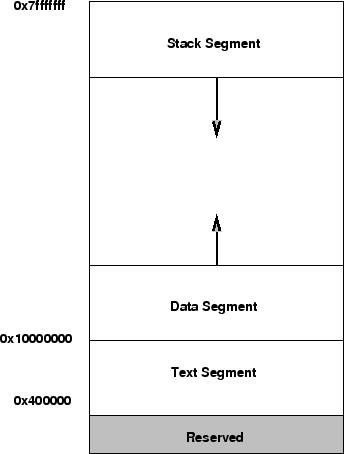
\includegraphics[width=\textwidth]{gmemory.png}
\end{figure}

\iffalse
Las arquitecturas MIPS siguen la filosofía RISC, por lo que cumplen con las siguientes directrices:
\item Es una arquitectura Load-Store, es decir, para operar con datos, estos deben cargarse desde
la memoria principal en registros internos de la CPU, donde quedan disponibles para operar con
ellos. Así, las únicas instrucciones que acceden a memoria principal son las de carga - almacenamiento.
Estando los datos en registros de la CPU, el acceso a ellos es muchísimo más rápido que si estuvieran en memoria principal.
\item Ya que las únicas instrucciones de acceso a memoria principal son las de carga - almacenamiento,
se dispone de pocos y sencillos modos de direccionamiento, lo que facilita
enormemente la decodificación de las instrucciones y la obtención de sus operandos.
\item La organización del formato de las instrucciones también es muy sencillo, lo que facilita su
decodificación, pues dispone de pocos formatos, compartiendo todos la misma longitud fija
de instrucción.
\item Ya que no se opera con los datos en memoria principal, se hace necesario disponer de un
generoso conjunto de registros generales para albergar los distintos datos del programa.
\fi










\subsection{Instrucciones soportadas}
rellenar
    
\section{Compilador}
\subsection{Formato ejecutable .mips}

En un archivo compilado se puede encontrar mucha más información que las instrucciones del programa que codifica, por lo tanto, su formato no sólo depende de la arquitectura, sino además del sistema operativo.

Nuestra MV utiliza el siguiente formato -creado por nosotros- al cual le asignamos extensión .mips.


ARCHIVO EJECUTABLE

- Header (12 bytes):

    4B : data-segment size (in Bytes)

    4B : text-segment size (in bytes)

    4B : main address

- Data Segment (<data-segment size>):

    Addresses start at 0x10000000

- Text Segment (<text-segment size>):

    Addresses start at 0x400000

Ver sección MV para mayor información sobre el mapeo de memoria".

\subsection{Lexer}
\subsection{Parser}
\subsection{Problemas encontrados}
    
   
\section{Máquina virtual}
\subsection{Introducción}
para emular el procesador vamos a mantener todos los registros en memoria y a
medida que se interpretan las instrucciones estos van modificandose.
para eso definimos a los registros como un array de 32 enteros de 32 bits
y 3 variables de enteros de 32 bits para  los registros LO, HI y PC.

la interpretación de las instrucciones se lleva a cabo primero decodificando
estas y mapeando su significado a una función respectiva.
\subsection{Mini SO ficticio}
\subsubsection{Mapeo de memoria}
Redactar bien

Text Segment starts at 0x400000
Data Segment starts at 0x10000000
Heap memory starts at 0x10010000
Stack memory ends at 0x7FFFFFFC
\subsubsection{Syscalls provistas}
Redactar bien

El argumento va en \texttt{\$v0} y las syscalls se enumeran de 1 a 12. ?

\subsection{Modulos}
\subsubsection{Syscalls}
Este modulo se encarga de la implementacion de las llamadas al sistema.

las siguientes syscalls han sido diseñadas e implementadas:

\begin{table}[H]
\centering
\begin{tabular}{@{}lc@{}}
\toprule
\multicolumn{1}{c}{Nombre} & Numero \\ \midrule
SC\_PRINT\_INTEGER                        & 1      \\
SC\_PRINT\_FLOAT                        & 2      \\
SC\_PRINT\_DOUBLE                        & 3      \\
SC\_PRINT\_STRING                       & 4      \\
SC\_READ\_INTEGER                        & 5      \\
SC\_READ\_FLOAT                        & 6      \\
SC\_READ\_DOUBLE                        & 7      \\
SC\_READ\_STRING                       & 8      \\
SC\_MALLOC                       & 9      \\
SC\_EXIT                       & 10      \\
SC\_PRINT\_CHAR                       & 11      \\
SC\_READ\_CHAR                       & 12      \\
\end{tabular}%
\end{table}

\subsubsection{Simulator}

Este modulo contiene las funciones necesarias para inicializar y resetar la maquina virtual. Ademas, implementa un pequeño \textit{shell} que permitirá correr los programas con mayor control sobre ellos. En particular, este modulo maneja los breakpoints. 

Las operaciones soportadas por el shell  son las siguientes:

\begin{table}[H]
\hskip-2.0cm
\begin{tabular}{@{}cll@{}}
\toprule
\multicolumn{1}{c}{Atajo} & Nombre                                                       & Acción                                                                        \\ \midrule
h                         & help                                                         & muestra esta tabla de comandos.                                               \\
l                         & load \textless nombre archivo\textgreater                  & abre el archivo indicado.                                                     \\
n                         & step                                                         & realiza un paso en la simulación.                                             \\
n                         & step \textless n\textgreater                                  & realiza n pasos de la simulación.                                             \\
r                         & run                                                          & continúa la ejecución hasta un punto de interrupción.                         \\
i                         & init                                                         & inicializa la máquina virtual para una segunda ejecución.                     \\
w                         & where                                                        & imprime el valor actual del reg. PC y la instrucción apuntada.    \\
b                         & break \textless lista de dirs\textgreater              & coloca puntos de interrupción en las dir. especificadas.               \\
b                         & break                                                        & muestra todos los puntos de interrupción actuales.                            \\
c                         & clear \textless lista de dirs\textgreater              & borra todos los puntos de interrupción de las direcciones indicadas.          \\
c                         & clear                                                        & borra todos los puntos de interrupción.                                       \\
g                         & ignore \textless n\textgreater                                & ignora n puntos de interrupción consecutivos.                                 \\
j                         & jump \textless dirección\textgreater                          & modifica el registro PC para que apunte a la dirección seleccionada.          \\
s                         & set \textless registro\textgreater \textless\%i\textgreater   & actualiza el valor del registro de prop. gral. con el valor dado.             \\
f                         & fset \textless registro\textgreater \textless\%f\textgreater  & actualiza el valor del registro de pto. flotante con el valor dado.           \\
d                         & dset \textless registro\textgreater \textless\%lf\textgreater & actualiza el valor de dos regs de pto. flotante con el doble dado. \\
p                         & print                                                        & imprime el valor de todos los registros (incluyendo PC, HI y LO)              \\
q                         & quit                                                         & apaga la máquina virtual.                                                    
\end{tabular}
\end{table}

\subsubsection{Regs}

Este modulo implementa los registros de propósito general ya introducidos anteriormente, como también los registros \texttt{\$f0 - \$f31} que pertenecen al coprocesador 1 y sirven para realizar operaciones con números de punto flotante, tanto en simple precision como en doble precision. En este ultimo caso, se utilizan dos registros en simultaneo para almacenar un único valor doble.

Por otro lado, este modulo hace los chequeos necesarios en tiempo de compilación para garantizar que la maquina virtual sea compilada en una plataforma que soporte el estándar IEE754, ya que de esta norma depende la correctitud de nuestro simulador.

\subsubsection{Memory}

Este modulo se encarga de administrar la memoria de la maquina virtual automáticamente: segmento de texto, de datos, heap y stack; como también de realizar la traducción de las direcciones virtuales que maneja el programa a direcciones "reales" de la maquina virtual (que por supuesto, son a su vez direcciones virtuales para la maquina host). Notemos que a pesar de que la primitiva malloc es un syscall, su implementacion (a través de un sbrk propio) esta implementada en este modulo.

\subsubsection{Instructions}

Este modulo es probablemente el corazón de la maquina virtual. Aquí se encuentran implementadas todas las instrucciones de MIPS I, en conjunto con una función \texttt{decode} que se encarga de tomar una instrucción compilada e interpretarla para poder ejecutar los comandos que ella describe. 

\subsubsection{Files}

La función de este modulo es sencilla: abrir un programa ejecutable para MIPS y cargarlo en la maquina virtual.


\subsection{Notas y problemas encontrados}
earlier this week:
	We don't understand how memory should be mapped in a multitask OS. We leave that aside. Our simulation is simplified so as to not need \($gp)\ register and alikes.

	We try to understand how to encode the data segment into an executable. We find out that depends on the OS and has nothng to do with MIPS architecture. We invent own our executable format.

	Does the PC always point to the current instruction? Yes. We dug into the matter and discovered the truth.

15/03:
	We add support for floating point types, we struggle trying to find a way to check during compilation time that the machine is compliant with IEEE754 standards.

18-19/03:
    Stack and Heap successfully virtualized!

20/03:
	Modified the executable's header to include the 'main' memory address (where the program starts).

26/03:
	Spent the whole day trying to discover a bug in the compiler which happened to be we had misopened a file in text mode rather than binarily.

\end{document}